\newpage
\section{Setting up your workspace}
\genHeader

Nowadays, \emph{no one} writes a complex parser completely by hand. Although this is sometimes still necessary for syntactically challenging languages, most
parsers can be quickly whipped up using context-free \emph{string grammars}\footnote{For simple cases, \emph{regular expressions} can also be used} that are
typically written in Extended Backus-Naur Form (EBNF)\define{EBNF}. ANTLR is a tool that can generate a parser from this compact specification for
a host of target programming languages, including Java. Although ANTLR might not be the most efficient or powerful parser generator, it's open-source, well
documented and supported, and allows for a pragmatic and elegant fallback to Java if things get nasty and we have to resort to some dirty tricks to get the job
done.

To set up your workspace for the model-to-text transformation, you have two options: (1) Import a cheat package with everything already
prepared (useful if you're just joining us), or (2) if you've worked through the previous part, continue with your existing
workspace. Both options will work, but note that all of our screenshots from now on assume that you chose Option (1), so don't let that irritate you.

As some of you are just reading this handbook without actually getting your hands dirty with an implementation (beware: no pain, no gain!), we have included a
screenshot of the dictionary metamodel that you get with both options in our visual (Fig.~\ref{ea:dictLang}) and textual (Fig.~\ref{eclipse:dictLangMetamodel})
concrete syntax.

\vspace{0.5cm}

% --- Dictionary metamodels --
\begin{figure}[htbp]
\begin{centering}
  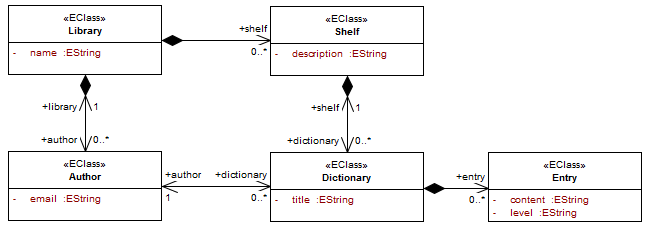
\includegraphics[width=\textwidth]{ea_dictionaryMetamodel}
  \caption{Metamodel for dictionaries (visual concrete syntax)}
  \label{ea:dictLang}
  \end{centering}
\end{figure}

\newpage

\begin{figure}[h!]
  \hspace{-1.5cm}
  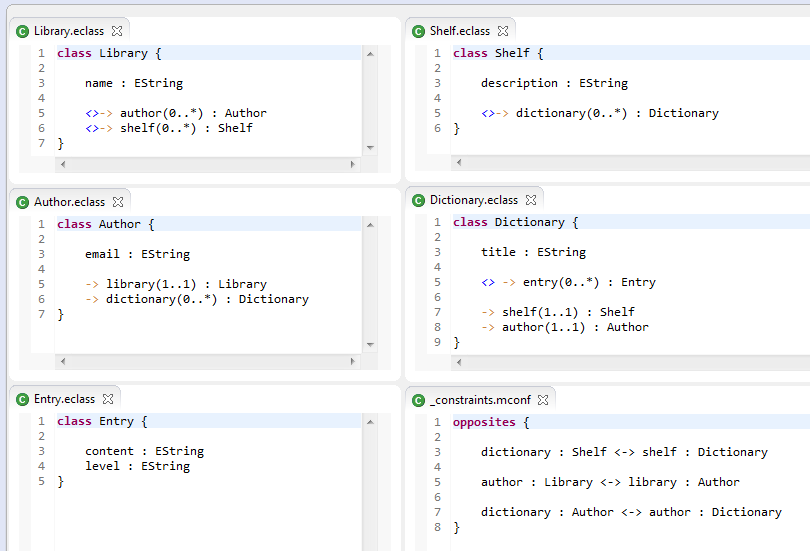
\includegraphics[width=1.2\textwidth]{eclipse_dictionaryMetamodel}
  \caption{Metamodel for dictionaries (textual concrete syntax)}
  \label{eclipse:dictLangMetamodel}
\end{figure}

\vspace{0.5cm}

% --- Option descriptions --
\begin{description}

\item[Option 1: Import a complete cheat package]

\item[$\blacktriangleright$] \hspace{0.3cm} Import the Part V `cheat package' by selecting ``New" in the toolbar, and the cheat package in the concrete syntax
of your choice (Fig.~\ref{eclipse_cheatPackage}).

\begin{figure}[htbp]
\begin{center}
  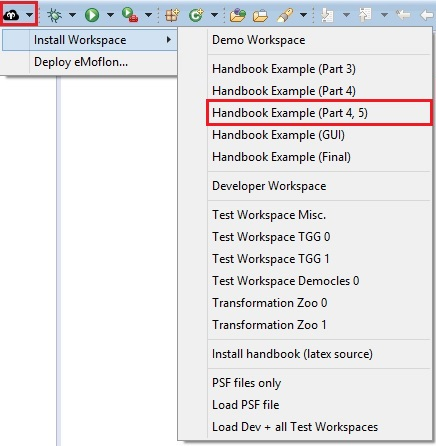
\includegraphics[width=0.65\textwidth]{eclipse_loadDictionaryProject}
  \caption{Load the cheat package for Part V into your workspace}
  \label{eclipse_cheatPackage}
\end{center}
\end{figure}

\vspace{0.5cm}

% -- Export/Import ---
\item[Option 2: Continue with the workspace from Part IV]


\item[$\blacktriangleright$] \hspace{0.3cm} Use the same metamodel for \texttt{Dictionary} as completed in Part IV. Just make sure you haven't radically changed
the dictionary metamodel (i.e., it still closely resembles the metamodel in either Fig.~\ref{ea:dictLang} or Fig.~\ref{eclipse:dictLangMetamodel}). Everything
else should work fine using the exact same workspace but remember, your screen may look different than our screenshots.

\end{description}


We recommend reviewing the dictionary metamodel until you feel comfortable with what you'll be working with. 

\newpage

\texttt{DictionaryLanguage} is only one of two metamodels that we'll be using to specify the TGG transformation. After all, TGGs typically require separate
source and target metamodels. The second metamodel involved in the transformation will be eMoflon's standard \texttt{MocaTree} language.\footnote{MOCA stands
for Moflon Code Adapter (not coffee, sorry.)} It basically combines concepts from a filesystem (folders and files), XML (text-only nodes and attributes), and a
general indexed containment hierarchy. It is provided by our Eclipse plugin and is automatically added to the build path, so it won't actually appear
anywhere in your Eclipse workspace.

Figure~\ref{mocaTreeMetamodel} is a visual depiction of this MocaTree model.\footnote{If you are using the visual syntax, feel free to view a detailed metamodel
by opening \texttt{dictionary.eap}, navigating to the \texttt{MocaTree} EPackage, and opening its diagram.} As you can see, the most important element is
\texttt{Node}. Note that a single \texttt{Node} can store any number of \texttt{Attribute} or \texttt{Text} elements (subnodes), but only belongs to one
\texttt{File}. If you look closer at \texttt{File}, you'll also notice that it belongs to a single \texttt{Folder}. \texttt{Folder} is able to store any number
of \texttt{File}s or subfolders.

\newpage

You can see that all elements inherit an \texttt{index} and \texttt{name} attribute. \texttt{Index} can be used to demand a certain \emph{order}
of nodes in a tree, otherwise not guaranteed by default (i.e., to enforce a hierarchy), while \texttt{name} can be any arbitrary string value. 

\vspace{1cm}

\begin{figure}[htbp]
  \begin{centering}
  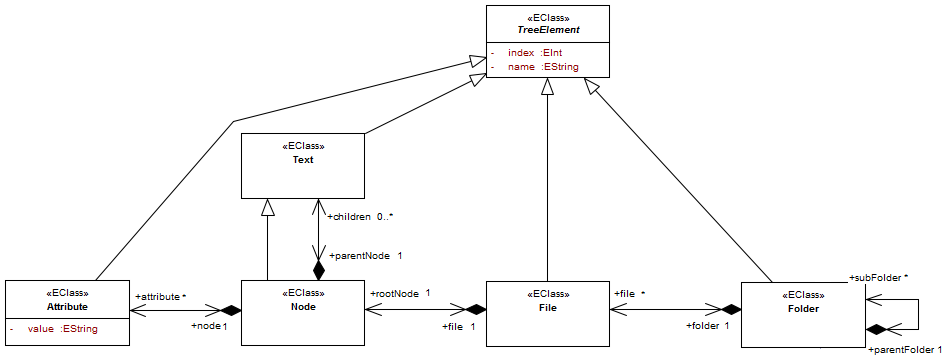
\includegraphics[width=\textwidth]{MocaTreeMetamodel}
  \caption{Visual depiction of the MocaTree metamodel}
  \label{mocaTreeMetamodel}
  \end{centering}
\end{figure}

\vspace{1cm}

Enough chatting -- let's begin by creating the TGG project that will implement our model-to-text transformation.

\jumpDual{initialize vis}{initialize tex}

\newpage

\newpage
\hypertarget{initialize vis}{}
\subsection{First steps}
\visHeader

\begin{itemize}

\item[$\blacktriangleright$] From your Eclipse workspace, open the \texttt{Dict\-ion\-ary.eap} file in Enterprise Architect (EA). The project browser should
closely resemble Fig.~\ref{ea:mocaTagged}. As you can see, the project is already populated with \texttt{MocaTree} and other built-in metamodels
in the \texttt{eMoflon Languages} working set.

\vspace{0.5cm}

\begin{figure}[htpb]
\begin{center}
  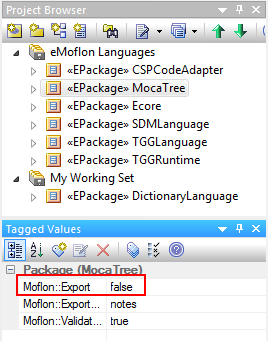
\includegraphics[width=0.4\textwidth]{ea_mocaTaggedValues}
  \caption{\texttt{MocaTree} is one of eMoflons' internal metamodels}
  \label{ea:mocaTagged}
\end{center}
\end{figure}

\end{itemize}

\vspace{-0.5cm}

If you inspect the tagged values\footnote{The ``Tagged Values'' window can be opened by going to ``View/Tagged Values'' or by hovering over the \texttt{Tagged
Values} tab immediately to the right of the project browser.} for these built-in languages, you'll notice that the \texttt{MocaTree} package has the
\texttt{Moflon::Export} value set to \texttt{false}. This ensures that the package is \emph{ignored} when exporting. As with all such standard metamodels (e.g.,
Ecore or our SDM metamodel) the \texttt{MocaTree} package in EA should be regarded as read-only, required only in the EA project so that SDMs/TGGs can refer to
the classes defined in the package.

\begin{itemize}

\item[$\blacktriangleright$] Despite \texttt{DictionaryLanguage} being contained in a different working set than \texttt{MocaTree}, the two
metamodels are contained within the same EA project (EAP) which means you are able to create a new TGG using them both. Add a new package to \texttt{My
Working Set} named \texttt{Dict\-ion\-ary\-Code\-Adap\-ter}.

\item[$\blacktriangleright$] Select the package and add a new TGG schema diagram as depicted in Fig.~\ref{ea:newTGGDiagram}. In the next dialogue window,
set the source project as \texttt{MocaTree}, and the target project as \texttt{Dict\-ion\-ary\-Lang\-uage}.

\begin{figure}[h!]
\begin{center}
  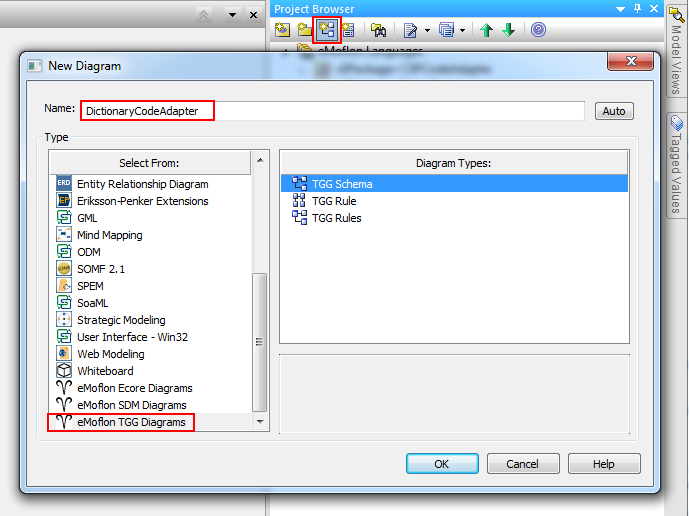
\includegraphics[width=0.9\textwidth]{ea_adapterTGGDiagram}
  \caption{Create a new TGG schema diagram}
  \label{ea:newTGGDiagram}
\end{center}
\end{figure}

\item[$\blacktriangleright$] For the moment, add a single correspondence type to the new diagram now active in the editor (the TGG \texttt{schema}) between
\texttt{Folder} and \texttt{Library}. Remember, you can get the classes by drag-and-dropping each element into the diagram, then quick-creating a new
\texttt{TGG Correspondence Type} between them.\footnote{For details on the correspondence metamodel and how to create types, refer to Part IV, Section 3.} Your diagram
should come to resemble Fig.~\ref{ea:firstCorrType}.

\vspace{0.5cm}

\begin{figure}[htpb]
\begin{center}
  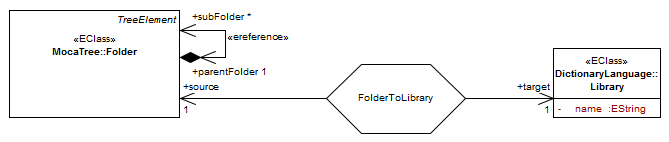
\includegraphics[width=\textwidth]{ea_firstAdapterCorrespondence}
  \caption{The first correspondence type for the transformation}
  \label{ea:firstCorrType}
\end{center}
\end{figure}

\newpage

\item[$\blacktriangleright$] Your complete project browser should now resemble Fig.~\ref{ea:TGGProjBrow}, where \texttt{Dict\-ion\-ary\-Code\-Adap\-ter} is now
explicitly listed as a \texttt{TGGSchemaPackage}.

\vspace{0.5cm}

\begin{figure}[htpb]
\begin{center}
  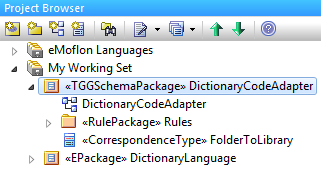
\includegraphics[width=0.5\textwidth]{ea_TGGProjectBrowser}
  \caption{A fully prepared TGG project}
  \label{ea:TGGProjBrow}
\end{center}
\end{figure}

\item[$\blacktriangleright$] Validate and export your file via the eMoflon control panel,\footnote{Activate via ``Extensions/Add-in Windows''} then switch
back to Eclipse and refresh the package explorer. A new \texttt{Dict\-ion\-ary\-Code\-Adap\-ter} project should appear in \texttt{My Working Set}.

\jumpSingle{subSec:setupParser}

\end{itemize}


\newpage
\hypertarget{M2TSettingUp tex}{}
\subsection{Initializing the project}
\texHeader

{\bf SELF:: update download so it includes a constraint file for \texttt{Dictionary}}
\begin{figure}[htbp]
\begin{center}
  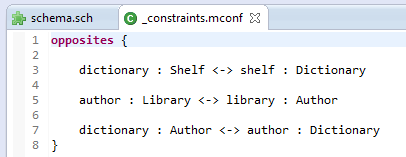
\includegraphics[width=0.7\textwidth]{eclipse_DOWNLOADUPDATE}
  \caption{SELF SELF}
\end{center}
\end{figure}

\begin{enumerate}

\item[$\blacktriangleright$] Your expanded \texttt{DictionaryLanguage} metamodel MOSL structure should resemble FIG. (starting point) You'll notice that it is
accessing the \emph{Moca} framework by importing the \texttt{MocaTree} in \texttt{\_imports.mconf}. (Explain, no screenshot?)

\item[$\blacktriangleright$] Right click on \texttt{MyWorkingSet} folder and create a new TGG. source: MocaTree. Target: DictionaryLanguage. FIG

\begin{figure}[htbp]
\begin{center}
  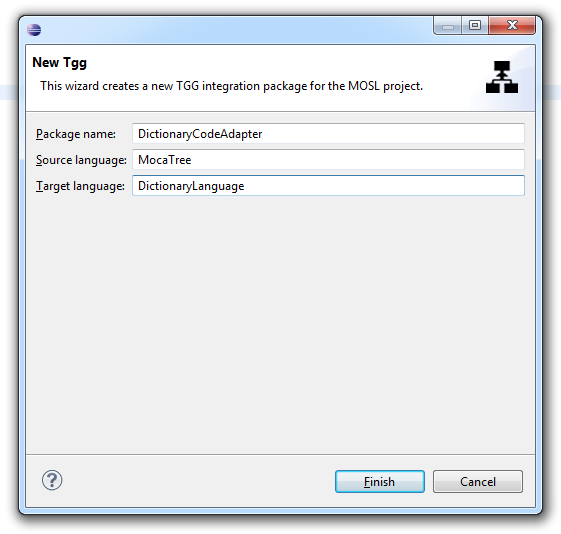
\includegraphics[width=0.9\textwidth]{eclipse_dictionaryCodeAdapterTGGProject}
  \caption{create tgg}
  \label{eclipse:newTGGProject}
\end{center}
\end{figure}


\item[$\blacktriangleright$] Before saving and building, initialize the correct generated code type by establishing the schema below (default is..)

\begin{figure}[htbp]
\begin{center}
  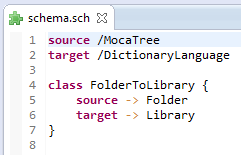
\includegraphics[width=0.5\textwidth]{eclipse_schemaStart}
  \caption{first rule}
  \label{eclipse:firstSchema}
\end{center}
\end{figure}

\item[$\blacktriangleright$] Save and build your project! Confirm a generated project was created in the \texttt{MyWorkingSet} node, and carry on!

\end{enumerate}


\newpage
\hypertarget{subSec:setupParser}{}
\subsection{Setting up the Parser}
\genHeader

\begin{itemize}

\item[$\blacktriangleright$] It should now resemble Fig.~\ref{eclipse:generatedAdapter}. Be sure to take a look at the \texttt{Moflon} and \texttt{Moca} library
nodes that reference jars for all required dependencies.

\begin{figure}[htpb]
\begin{center}
  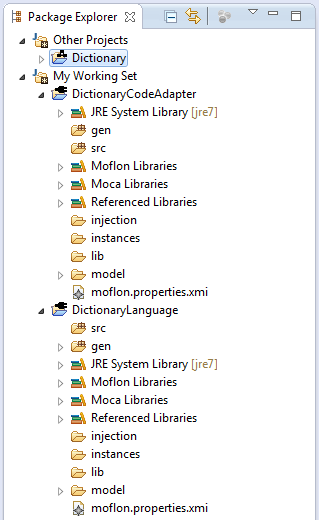
\includegraphics[width=0.4\textwidth]{eclipse_generatedAdapter}
  \caption{figureCaption}
  \label{eclipse:generatedAdapter}
\end{center}
\end{figure}

\item[$\blacktriangleright$] Right-click on \texttt{DictionaryCodeAdapter} and navigate to ``eMolfon/ Add Parser/Unparser'' (Fig~\ref{eclipse:contextParser}).

\begin{figure}[htpb]
\begin{center}
  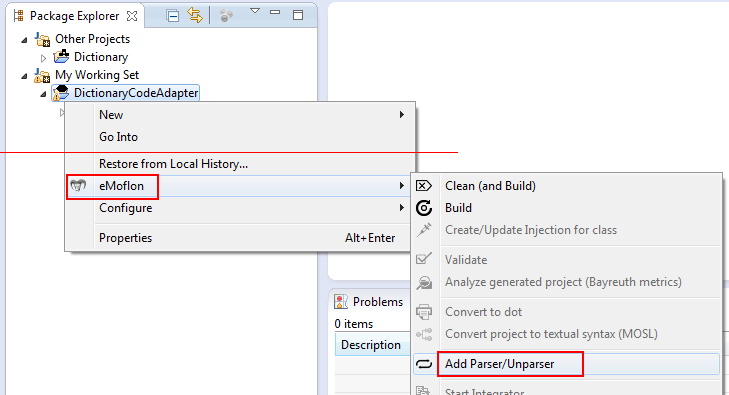
\includegraphics[width=0.9\textwidth]{eclipse_contextAddParserUnparser}
  \caption{figureCaption}
  \label{eclipse:contextParser}
\end{center}
\end{figure}

\item[$\blacktriangleright$] In the wizard dialogue (Fig~\ref{eclipse:wizardParser}), enter ``dictionary'' as the \texttt{File extension}, and make sure
the boxes \texttt{Create Parser} and \texttt{Create Unparser} with \texttt{ANTLR} are chosen as corresponding technology in both cases. Click \texttt{Finish} to
close.

\begin{figure}[htpb]
\begin{center}
  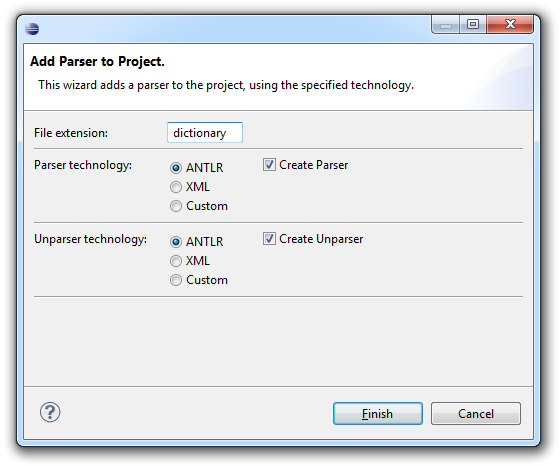
\includegraphics[width=0.8\textwidth]{eclipse_wizardParser}
  \caption{figureCaption}
  \label{eclipse:wizardParser}
\end{center}
\end{figure}

If everything has been installed and set up properly, parser and unparser stubs should be generated and \texttt{ANTLR} should automatically build the
corresponding Java code as depicted in Fig.~\ref{eclipse:generatedParser}.

\begin{figure}[htpb]
\begin{center}
  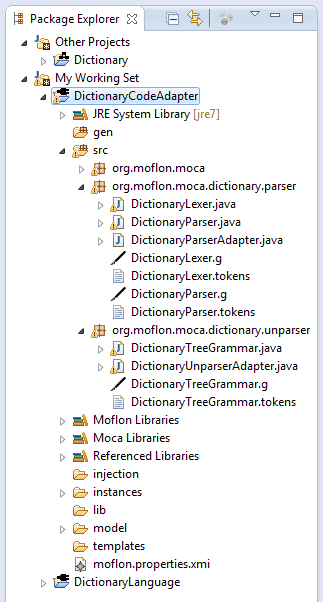
\includegraphics[width=0.4\textwidth]{eclipse_generatedParser}
  \caption{figureCaption}
  \label{eclipse:generatedParser}
\end{center}
\end{figure}

\end{itemize}

